%% ===========================================
%% Nation-wise Failure Distribution
%% Version 9 - Using after end axis for labels
%% ===========================================

\documentclass[tikz,border=5pt]{standalone}
\usepackage{tikz}
\usepackage{pgfplots}
\pgfplotsset{compat=1.18}
\usetikzlibrary{calc, positioning, arrows.meta, decorations.pathreplacing}

% Colorblind-safe palette (Okabe-Ito based)
\definecolor{c_nonlatin}{RGB}{230,159,0}    % orange
\definecolor{c_ocr}{RGB}{86,180,233}        % sky blue
\definecolor{c_math}{RGB}{204,121,167}      % reddish purple
\definecolor{c_reason}{RGB}{0,114,178}      % strong blue
\definecolor{c_other}{RGB}{180,180,180}     % neutral gray

\begin{document}

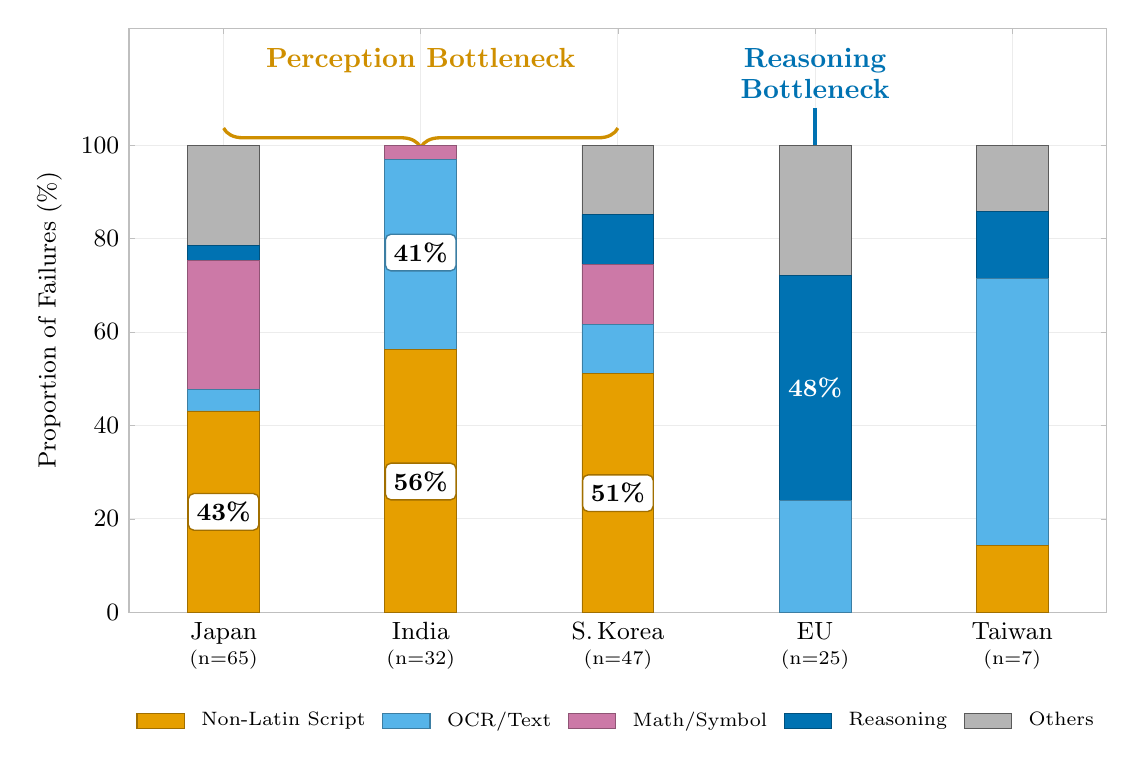
\begin{tikzpicture}
\begin{axis}[
    ybar stacked,
    bar width=26pt,
    width=14cm,
    height=9cm,
    ylabel={Proportion of Failures (\%)},
    ymin=0,
    ymax=125,
    ytick={0,20,40,60,80,100},
    xtick=data,
    symbolic x coords={Japan, India, S.Korea, EU, Taiwan},
    xticklabels={
        {Japan\\[-2pt]{\scriptsize(n=65)}},
        {India\\[-2pt]{\scriptsize(n=32)}},
        {S.\,Korea\\[-2pt]{\scriptsize(n=47)}},
        {EU\\[-2pt]{\scriptsize(n=25)}},
        {Taiwan\\[-2pt]{\scriptsize(n=7)}}
    },
    xticklabel style={align=center, font=\small},
    y tick label style={font=\small},
    ylabel style={font=\small},
    legend style={
        at={(0.5,-0.15)},
        anchor=north,
        legend columns=5,
        font=\scriptsize,
        column sep=4pt,
        draw=none,
    },
    legend cell align={left},
    enlarge x limits=0.12,
    clip=false,
    grid=major,
    major grid style={gray!15, line width=0.3pt},
    axis line style={gray!50},
    tick style={gray!50},
    major tick length=2pt,
    % Store coordinates for later use
    after end axis/.code={
        % Japan: Non-Latin 43%
        \draw (axis cs:Japan, 21.5) node[font=\small\bfseries, text=black, 
              fill=white, inner sep=3pt, rounded corners=2pt,
              draw=c_nonlatin!70!black, line width=0.5pt] {43\%};
        % India: Non-Latin 56%
        \draw (axis cs:India, 28) node[font=\small\bfseries, text=black,
              fill=white, inner sep=3pt, rounded corners=2pt,
              draw=c_nonlatin!70!black, line width=0.5pt] {56\%};
        % India: OCR 41%
        \draw (axis cs:India, 77) node[font=\small\bfseries, text=black,
              fill=white, inner sep=3pt, rounded corners=2pt,
              draw=c_ocr!70!black, line width=0.5pt] {41\%};
        % S.Korea: Non-Latin 51%
        \draw (axis cs:S.Korea, 25.5) node[font=\small\bfseries, text=black,
              fill=white, inner sep=3pt, rounded corners=2pt,
              draw=c_nonlatin!70!black, line width=0.5pt] {51\%};
        % EU: Reasoning 48%
        \draw (axis cs:EU, 48) node[font=\small\bfseries, text=white] {48\%};
    },
]

% Non-Latin Script (orange)
\addplot+[
    ybar stacked,
    fill=c_nonlatin,
    draw=c_nonlatin!70!black,
    line width=0.3pt,
    forget plot,
] coordinates {
    (Japan, 43.1)
    (India, 56.3)
    (S.Korea, 51.1)
    (EU, 0)
    (Taiwan, 14.3)
};

% OCR/Text Recognition (sky blue)
\addplot+[
    ybar stacked,
    fill=c_ocr,
    draw=c_ocr!70!black,
    line width=0.3pt,
    forget plot,
] coordinates {
    (Japan, 4.6)
    (India, 40.6)
    (S.Korea, 10.6)
    (EU, 24.0)
    (Taiwan, 57.1)
};

% Math/Symbol (reddish purple)
\addplot+[
    ybar stacked,
    fill=c_math,
    draw=c_math!70!black,
    line width=0.3pt,
    forget plot,
] coordinates {
    (Japan, 27.7)
    (India, 3.1)
    (S.Korea, 12.8)
    (EU, 0)
    (Taiwan, 0)
};

% Pure Reasoning (strong blue)
\addplot+[
    ybar stacked,
    fill=c_reason,
    draw=c_reason!70!black,
    line width=0.3pt,
    forget plot,
] coordinates {
    (Japan, 3.1)
    (India, 0)
    (S.Korea, 10.6)
    (EU, 48.0)
    (Taiwan, 14.3)
};

% Others (neutral gray)
\addplot+[
    ybar stacked,
    fill=c_other,
    draw=c_other!50!black,
    line width=0.3pt,
    forget plot,
] coordinates {
    (Japan, 21.5)
    (India, 0)
    (S.Korea, 14.9)
    (EU, 28.0)
    (Taiwan, 14.3)
};

% Manual legend (horizontal)
\addlegendimage{area legend, fill=c_nonlatin, draw=c_nonlatin!70!black}
\addlegendentry{Non-Latin Script}
\addlegendimage{area legend, fill=c_ocr, draw=c_ocr!70!black}
\addlegendentry{OCR/Text}
\addlegendimage{area legend, fill=c_math, draw=c_math!70!black}
\addlegendentry{Math/Symbol}
\addlegendimage{area legend, fill=c_reason, draw=c_reason!70!black}
\addlegendentry{Reasoning}
\addlegendimage{area legend, fill=c_other, draw=c_other!50!black}
\addlegendentry{Others}

% ===== Bottleneck annotations =====

% Perception Bottleneck brace (Japan to S.Korea)
\draw[decorate, decoration={brace, amplitude=7pt, mirror, raise=4pt}, 
      very thick, c_nonlatin!90!black]
    (axis cs:Japan, 106) -- (axis cs:S.Korea, 106);
\node[font=\normalsize\bfseries, c_nonlatin!90!black] 
    at (axis cs:India, 118) {Perception Bottleneck};

% Reasoning Bottleneck (centered above EU bar)
\node[font=\normalsize\bfseries, c_reason] 
    at (axis cs:EU, 118) {Reasoning};
\node[font=\normalsize\bfseries, c_reason] 
    at (axis cs:EU, 112) {Bottleneck};
\draw[-{Stealth[length=6pt, width=5pt]}, line width=1.2pt, c_reason]
    (axis cs:EU, 108) -- (axis cs:EU, 75);

\end{axis}
\end{tikzpicture}

\end{document}
